% ============================================================
%  QAOA for MaxCut — Beamer Presentation
%  Sehong Park & Adolfo Menendez Rua
%  Physics 565 / 656 · Spring 2026
% ============================================================
%
%  Compile with:    latexmk -pdf qaoa_presentation.tex
%  Or:              pdflatex qaoa_presentation.tex (twice)
%
%  Requires the Metropolis theme. If not installed:
%      tlmgr install beamertheme-metropolis
%  Or use Overleaf, where it ships by default.
% ============================================================

\documentclass[aspectratio=169,11pt]{beamer}

% ----- Theme -------------------------------------------------
\usetheme{metropolis}
\usecolortheme{default}
\metroset{
  numbering=fraction,
  progressbar=frametitle,
  block=fill,
  sectionpage=progressbar,
  subsectionpage=progressbar
}

% ----- Color palette (matches the original PDF) --------------
\definecolor{NavyDeep}{HTML}{1B3A4B}
\definecolor{NavyMid} {HTML}{2E86C1}
\definecolor{NavyLite}{HTML}{AED6F1}
\definecolor{Mustard} {HTML}{D68910}
\definecolor{Cream}   {HTML}{FBF8F2}
\definecolor{Crimson} {HTML}{C0392B}
\definecolor{Forest}  {HTML}{27AE60}

\setbeamercolor{normal text}{fg=NavyDeep,bg=Cream}
\setbeamercolor{alerted text}{fg=Mustard}
\setbeamercolor{frametitle}{bg=NavyDeep,fg=Cream}
\setbeamercolor{progress bar}{fg=Mustard,bg=NavyLite}
\setbeamercolor{title separator}{fg=Mustard}
\setbeamercolor{section in head/foot}{bg=NavyDeep,fg=Cream}
\setbeamercolor{block title}{bg=NavyDeep,fg=Cream}
\setbeamercolor{block body}{bg=NavyLite!25,fg=NavyDeep}

% ----- Packages ----------------------------------------------
\usepackage{amsmath,amssymb,amsthm}
\usepackage{bm}
\usepackage{graphicx}
\usepackage{booktabs}
\usepackage{array}
\usepackage{colortbl}
\usepackage{tikz}
\usepackage{xcolor}
\usepackage{pifont}
\usetikzlibrary{positioning,arrows.meta,shapes,fit,backgrounds}

% ----- Math shortcuts ---------------------------------------
\newcommand{\ket}[1]{\left|#1\right\rangle}
\newcommand{\bra}[1]{\left\langle#1\right|}
\newcommand{\braket}[2]{\left\langle#1\middle|#2\right\rangle}
\newcommand{\expval}[1]{\left\langle#1\right\rangle}
\renewcommand{\Re}{\mathrm{Re}}

% Convenience
\newcommand{\HC}{H_{C}}
\newcommand{\HB}{H_{B}}
\newcommand{\UC}{U_{C}}
\newcommand{\UB}{U_{B}}
\newcommand{\Sbar}{\overline{S}}
\newcommand{\pcx}{p_{cx}}

% ----- Title --------------------------------------------------
\title{QAOA for MaxCut}
\subtitle{The Quantum Approximate Optimization Algorithm}
\author{Sehong Park}
\institute{Physics 565 / 656 \ \textperiodcentered\  Spring 2026}
\date{}

% ============================================================
\begin{document}
% ============================================================

% ---- Title slide --------------------------------------------
\begin{frame}[plain]
  \titlepage
  \vspace{-1.5em}
  \begin{flushleft}
    {\footnotesize\color{NavyDeep!70}
      01 \,\textperiodcentered\, Introduction \quad
      02 \,\textperiodcentered\, Motivation  \quad
      03 \,\textperiodcentered\, Theory \quad
      04 \,\textperiodcentered\, Implementation \quad
      05 \,\textperiodcentered\, Results}
  \end{flushleft}
\end{frame}

% ============================================================
\section{Introduction}
% ============================================================

\begin{frame}{Definition of a graph}
  \framesubtitle{A finite vertex set plus a set of unordered pairs}
  \begin{columns}[T,onlytextwidth]
    \column{0.55\textwidth}
      \textbf{Vertex set}\\[2pt]
      $V = \{0, 1, 2, 3\}, \quad |V| = n = 4$
      \vspace{1.2em}

      \textbf{Edge set}\\[2pt]
      $E \subseteq \binom{V}{2}
        = \big\{\{0,1\},\{1,2\},\{2,3\},\{0,3\}\big\}$
      \vspace{1.5em}

      \begin{block}{Notation}
        Throughout: $n = |V|$ qubits, $m = |E|$ edges.\\
        Cuts will be encoded as bitstrings $z \in \{0,1\}^n$.
      \end{block}

    \column{0.42\textwidth}
      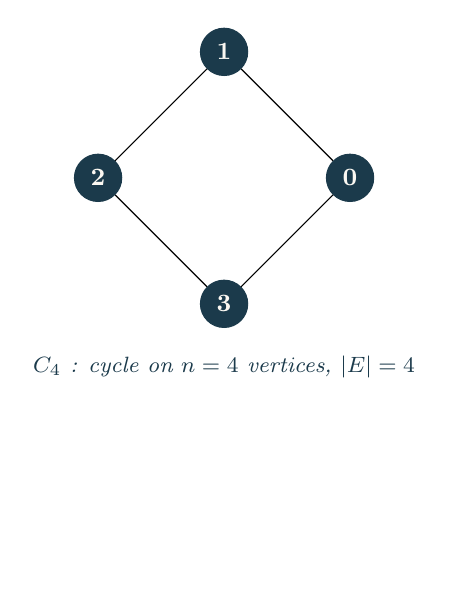
\begin{tikzpicture}[
          every node/.style={circle,draw=NavyDeep,fill=NavyDeep,
                             text=Cream,inner sep=2pt,minimum size=6mm,
                             font=\small\bfseries},
          every edge/.style={draw=NavyDeep,thick}]
        \node (1) at ( 0, 1.6) {1};
        \node (2) at (-1.6, 0) {2};
        \node (0) at ( 1.6, 0) {0};
        \node (3) at ( 0,-1.6) {3};
        \draw (1)--(2) (2)--(3) (3)--(0) (0)--(1);
        \node[draw=none,fill=none,text=NavyDeep,font=\footnotesize\itshape]
            at (0,-2.4) {$C_4$ : cycle on $n=4$ vertices, $|E|=4$};
      \end{tikzpicture}
  \end{columns}
\end{frame}

% --- MaxCut definition (single combined slide) ----------------
\begin{frame}{The MaxCut problem}
  \framesubtitle{Partition $V = S \sqcup \Sbar$ to maximise the number of cut edges}

  \[
    C(S) \;=\; \big|\{(i,j)\in E : i\in S,\; j\in \Sbar\}\big|,
    \qquad
    S^{\star} \in \arg\max_{S\subseteq V} C(S).
  \]

  \vspace{-0.3em}
  \begin{center}
    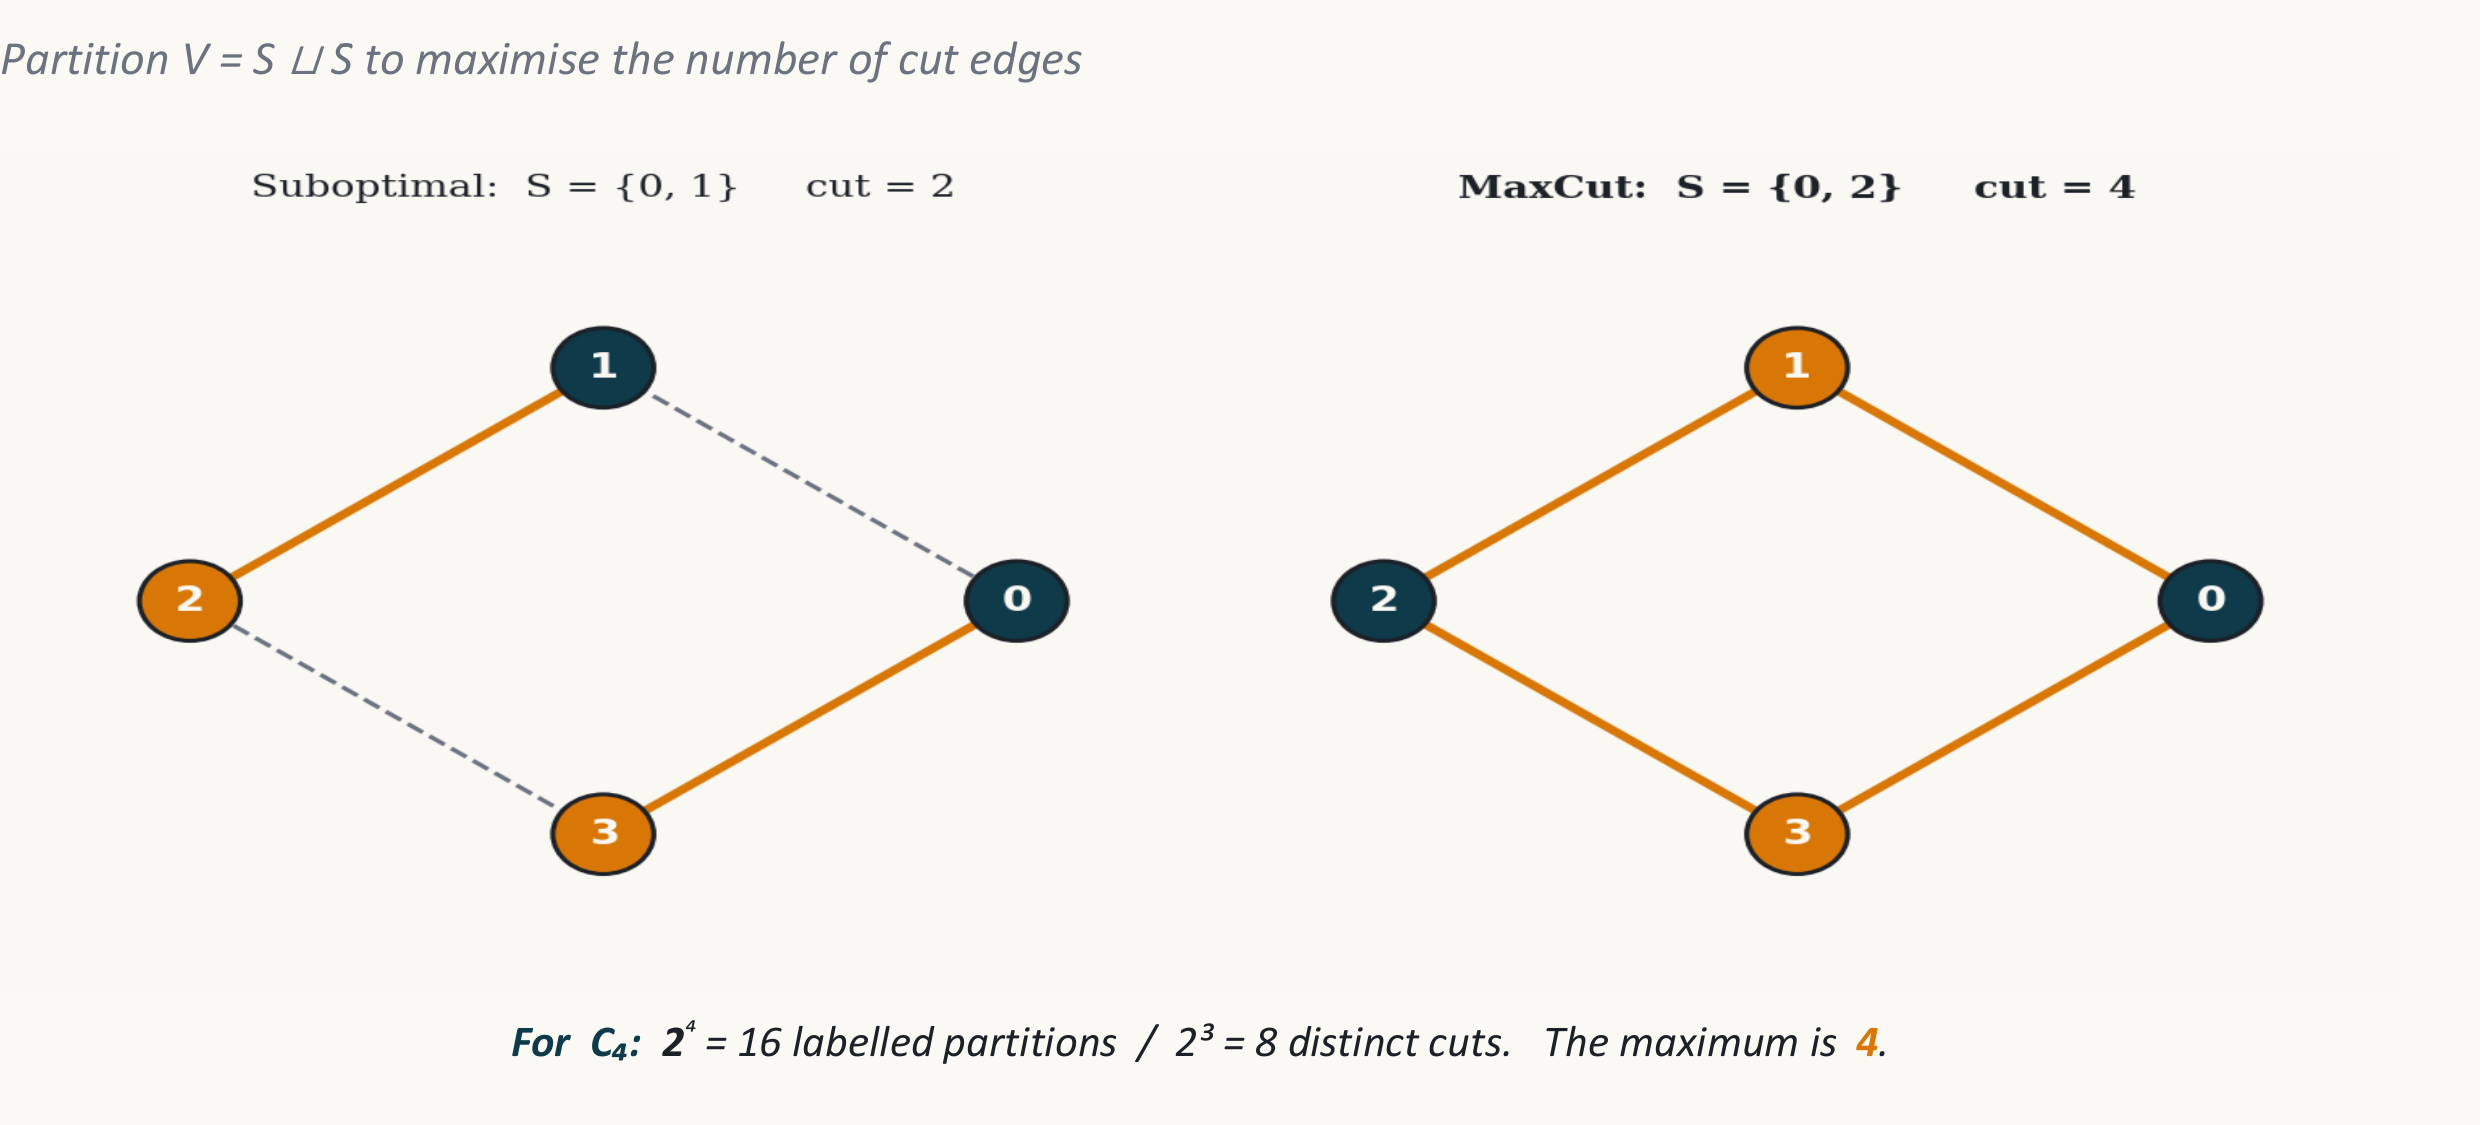
\includegraphics[width=0.95\textwidth]{figs_from_pdf/maxcut_problem.png}
  \end{center}

  \vspace{-0.5em}
  \footnotesize NP-hard (Karp 1972). \,Brute force: $2^n$ partitions.
  \,Best polynomial-time guarantee: GW $\geq 0.8786$ (1995).
\end{frame}

% ============================================================
\section{Motivation}
% ============================================================

% --- Portfolio Slide 1: setup --------------------------------
\begin{frame}{A worked example: portfolio diversification (1/2)}
  \framesubtitle{From financial intuition to a graph}
  \begin{columns}[T,onlytextwidth]
    \column{0.48\textwidth}
      \footnotesize
      \textbf{The investor's problem.}\\
      Hold $n$ assets with daily returns $r_i(t)$.
      \emph{Risk concentrates when assets move together} — so split the
      portfolio into two halves $S, \Sbar$, each \emph{internally
      uncorrelated}, so a shock to one asset does not drag the rest of
      its half with it.

      \vspace{0.5em}
      \textbf{Measure correlation.}
      \[
        \rho_{ij} \;=\; \frac{\mathrm{Cov}(r_i,r_j)}{\sigma_i\,\sigma_j}
        \;\in\; [-1,1]
      \]

      \vspace{0.3em}
      \textbf{Build the correlation graph.}
      \begin{itemize}\setlength{\itemsep}{1pt}
        \item Vertex $\leftrightarrow$ asset.
        \item Edge $(i,j)$ if $|\rho_{ij}| > 0.25$.
        \item Same-sector pairs $\Rightarrow$ thick edges
              ($\rho \approx 0.87$).
      \end{itemize}

    \column{0.50\textwidth}
      \centering
      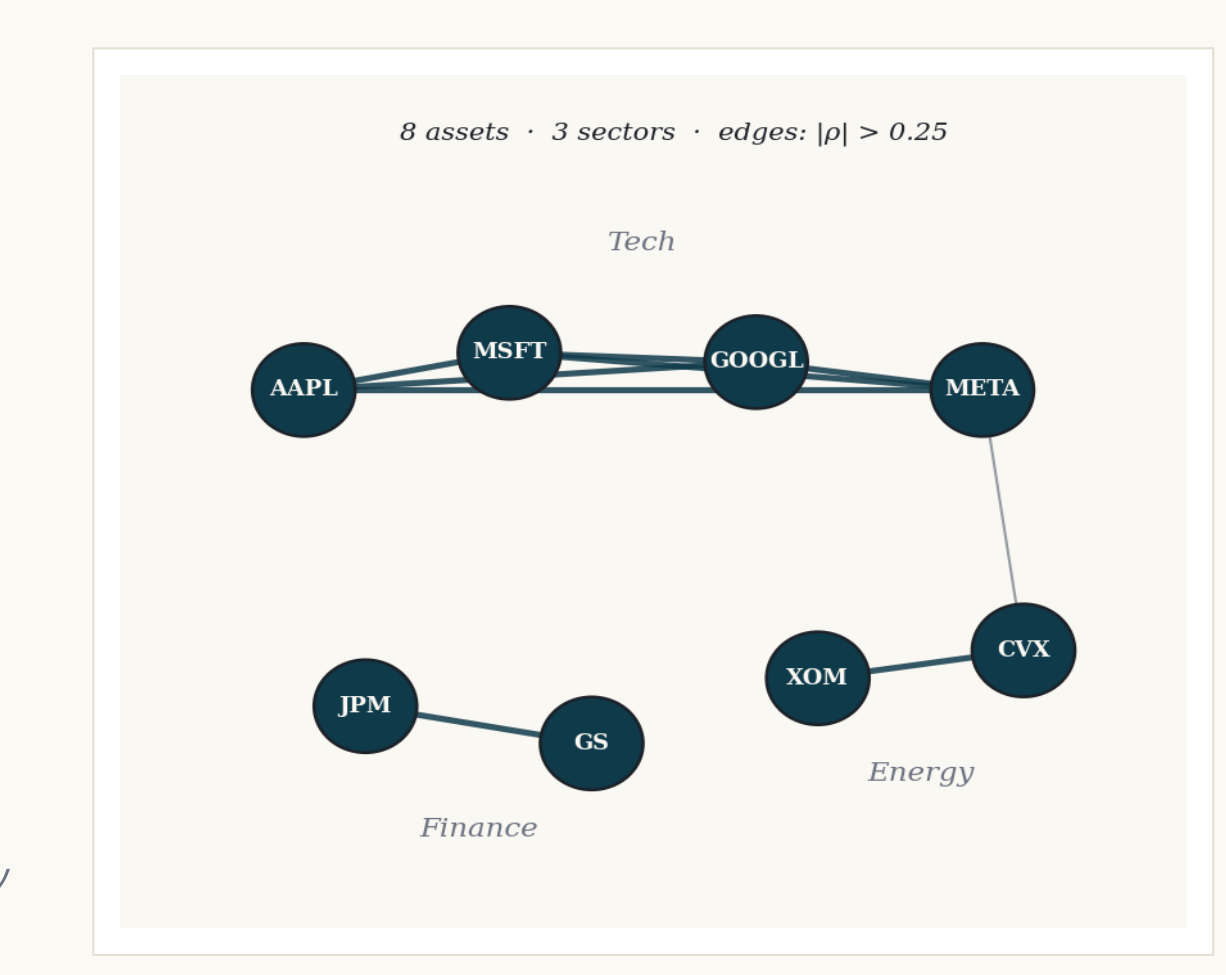
\includegraphics[width=\linewidth]{figs_from_pdf/portfolio_setup.png}\\[1pt]
      {\footnotesize\itshape 8 assets, 3 sectors --- intra-sector edges
       dominate.}
  \end{columns}
\end{frame}

% --- Portfolio Slide 2: solution ------------------------------
\begin{frame}{A worked example: portfolio diversification (2/2)}
  \framesubtitle{MaxCut on the correlation graph $\Rightarrow$ diversified split}
  \begin{columns}[T,onlytextwidth]
    \column{0.50\textwidth}
      \centering
      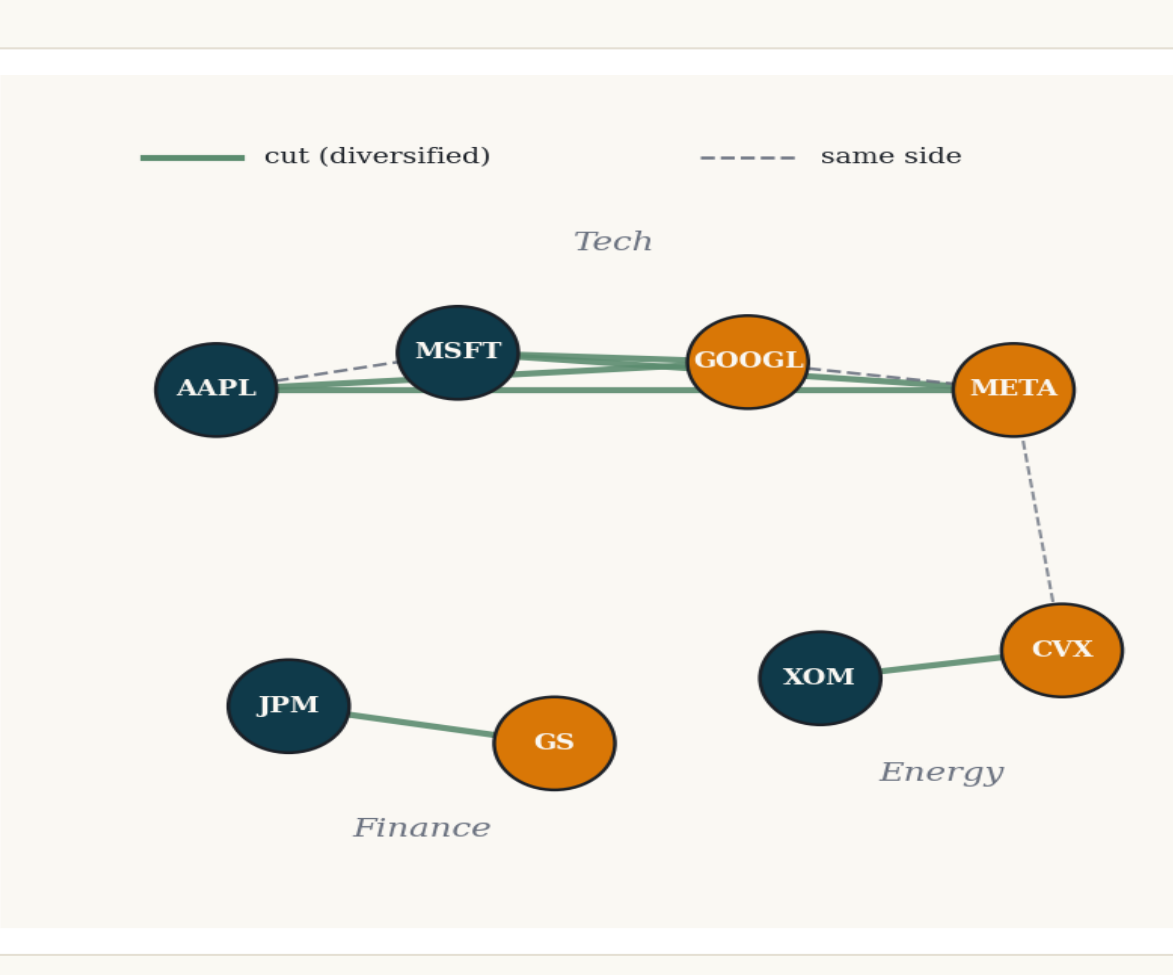
\includegraphics[width=\linewidth]{figs_from_pdf/portfolio_solved.png}\\[1pt]
      {\footnotesize\itshape Cut edges (green) separate correlated pairs;
       same-side edges (dashed) are correlations within a group.}

    \column{0.48\textwidth}
      \footnotesize
      \textbf{Result on the 8-asset example.}\\
      Group $S$ = \{AAPL, MSFT, JPM, XOM\},\\
      Group $\Sbar$ = \{GOOGL, META, GS, CVX\}.\\
      Each group contains one asset from every sector --- automatic
      sector diversification.

      \vspace{0.5em}
      \begin{tabular}{lc}
        \toprule
        Strategy & Avg.\ $|\rho|$ within group \\
        \midrule
        Na\"ive (Tech \,$|$\, Fin+Energy) & $0.87 \,/\, 0.32$ \\
        \rowcolor{NavyLite!25}\textbf{MaxCut} & $\mathbf{0.22 \,/\, 0.26}$ \\
        \bottomrule
      \end{tabular}

      \vspace{0.4em}
      \alert{$\sim\!4\times$ less correlated} inside each group.

      \vspace{0.4em}
      {\scriptsize\itshape\color{NavyDeep!70}
       Stylised: we threshold at $|\rho|>0.25$ and ignore expected
       returns and budget constraints --- the point is that
       ``diversification'' maps onto a cut.}
  \end{columns}
\end{frame}

% ============================================================
\section{Theory}
% ============================================================

\begin{frame}{From bitstring to Hamiltonian}
  \framesubtitle{Three steps: decision variable $\to$ spin $\to$ Pauli operator}
  \begin{columns}[T,onlytextwidth]
    \column{0.55\textwidth}
      \textbf{1.\ Decision variable}\\
      $z_i\in\{0,1\}$ with rule
      $z_i=0\Leftrightarrow i\in S$, $z_i=1\Leftrightarrow i\in\Sbar$.\\[4pt]
      Cut size: $C(z) = \sum_{(i,j)\in E}\mathbf{1}[z_i\neq z_j]$.

      \vspace{0.6em}
      \textbf{2.\ Rewrite with spins} $s_i = 1 - 2z_i\in\{+1,-1\}$:
      \[
        \mathbf{1}[z_i\neq z_j] \;=\; \tfrac{1}{2}(1 - s_i s_j).
      \]

      \vspace{0.6em}
      \textbf{3.\ Quantise} $s_i\to Z_i$ (Pauli-Z on qubit $i$):
      \[
        \boxed{\;\HC \;=\; \sum_{(i,j)\in E}\tfrac{1}{2}\bigl(I - Z_i Z_j\bigr)\;}
      \]

    \column{0.42\textwidth}
      \begin{block}{Key property}
        $\HC$ is \emph{diagonal} in the computational basis:
        \[
          \HC\ket{z} = C(z)\,\ket{z}.
        \]
        So $\langle\HC\rangle$ is the expected cut value, and the
        ground states are the MaxCut bitstrings.
      \end{block}
      \begin{alertblock}{Goal}
        Prepare $\ket{\psi}$ that maximises
        $\langle\psi|\HC|\psi\rangle$.
      \end{alertblock}
  \end{columns}
\end{frame}

\begin{frame}{What we are looking for}
  \framesubtitle{A bitstring that encodes a MaxCut partition --- shown on $C_4$}
  \begin{block}{Measurement rule}
    Measuring $\ket{\psi}$ in the computational basis returns
    $z = z_0 z_1 \cdots z_{n-1}$.
    Read out: $z_i = 0 \Rightarrow i\in S$, $\ z_i = 1 \Rightarrow i\in\Sbar$.
  \end{block}

  \vspace{0.4em}
  \centering
  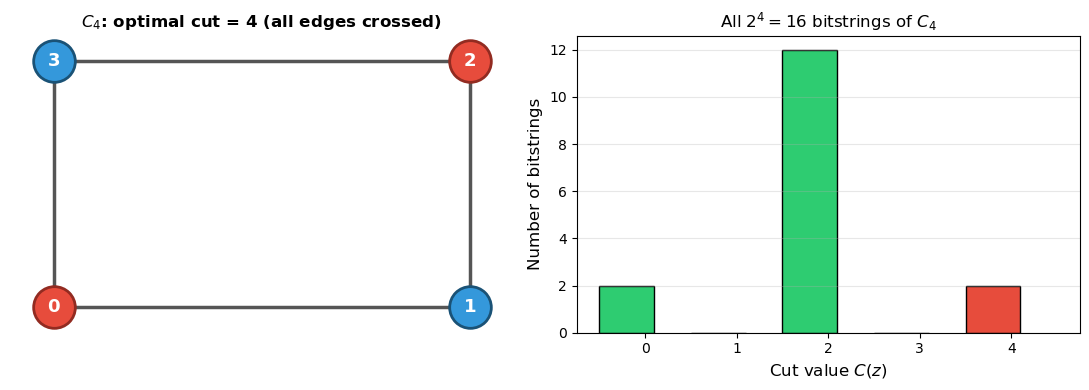
\includegraphics[width=\linewidth,height=0.62\textheight,keepaspectratio]{../Theory/figures/c4_maxcut.png}\\[2pt]
  {\footnotesize\itshape Goal: maximise the probability of sampling
   $\ket{1010}$ or $\ket{0101}$ --- the two MaxCut solutions of $C_4$.}
\end{frame}

\begin{frame}{Starting state: $\ket{+}^{\otimes n}$}
  \framesubtitle{Four reasons this is the natural initial state for QAOA}
  \begin{block}{}
    \[
      \ket{+}^{\otimes n}
      = \tfrac{1}{\sqrt{2^n}}\sum_{z\in\{0,1\}^n}\ket{z}
      = H^{\otimes n}\ket{0}^{\otimes n}.
    \]
  \end{block}
  \begin{columns}[T,onlytextwidth]
    \column{0.5\textwidth}
      \textbf{1.\ Uniform over candidates.}
      Equal weight on all $2^n$ bitstrings — no partition is preferred a priori.

      \vspace{0.5em}
      \textbf{2.\ Aligned with the mixer.}
      $X\ket{+}=+\ket{+}$, so $\HB = \sum_k X_k$ has $\ket{+}^{\otimes n}$
      as its top eigenstate.

    \column{0.5\textwidth}
      \textbf{3.\ Cheap to prepare.}
      One Hadamard per qubit --- constant-depth circuit from $\ket{0}^{\otimes n}$.

      \vspace{0.5em}
      \textbf{4.\ Adiabatic starting point.}
      Ground state of $H(t=0)=\HB$ in the adiabatic interpolation
      $H(t)=(1-t/T)\HB + (t/T)\HC$.
  \end{columns}
\end{frame}

\begin{frame}{The QAOA ansatz}
  \framesubtitle{Alternating layers of cost and mixer unitaries (Farhi et al.\ 2014)}
  \begin{block}{State}
    \[
      \ket{\psi_p(\bm\gamma,\bm\beta)} \;=\;
      \UB(\beta_p)\UC(\gamma_p)\cdots \UB(\beta_1)\UC(\gamma_1)\,
      \ket{+}^{\otimes n}
    \]
  \end{block}

  \begin{columns}[T,onlytextwidth]
    \column{0.5\textwidth}
      \textbf{Cost unitary}
      \[
        \UC(\gamma) = e^{-i\gamma \HC}
        \;=\; \prod_{(i,j)\in E} e^{-i\gamma(I-Z_i Z_j)/2}
      \]
      Encodes problem structure --- entangling.

    \column{0.5\textwidth}
      \textbf{Mixer unitary}
      \[
        \UB(\beta) = e^{-i\beta \HB},\quad \HB=\sum_k X_k
      \]
      Drives transitions between bitstrings --- single-qubit only.
  \end{columns}

  \vspace{0.4em}
  \begin{itemize}
    \item Depth $p$ \;\(\Rightarrow\)\; $2p$ variational parameters.
    \item Larger $p$: more expressive, but harder to optimise and noisier.
  \end{itemize}
\end{frame}

% --- Classical benchmarks (now also defines approximation ratio) ----
\begin{frame}{Classical benchmarks: greedy and Goemans--Williamson}
  \framesubtitle{Approximation ratio
    $r = \langle\psi|\HC|\psi\rangle / \mathrm{MaxCut}(G) \in [0,1]$}
  \begin{columns}[T,onlytextwidth]
    \column{0.46\textwidth}
      \footnotesize
      \textbf{Greedy.} Process vertices in order; each joins the side
      cutting more already-assigned edges. Worst-case $r=1/2$.

      \vspace{0.5em}
      \textbf{Greedy best-of-5.} Run greedy 5 times with different
      orderings; keep the best cut.

      \vspace{0.5em}
      \textbf{Goemans--Williamson (1995).} Relax to unit vectors,
      solve an SDP, round by a random hyperplane.
      Worst-case $r \geq 0.8786$, runtime $O(n^{3.5})$.

      \vspace{0.5em}
      \textbf{NP-hardness wall.}
      Achieving $r > 16/17 \approx 0.941$ in polynomial time would
      imply $\mathrm{P}=\mathrm{NP}$ (H{\aa}stad 2001).

    \column{0.52\textwidth}
      \centering
      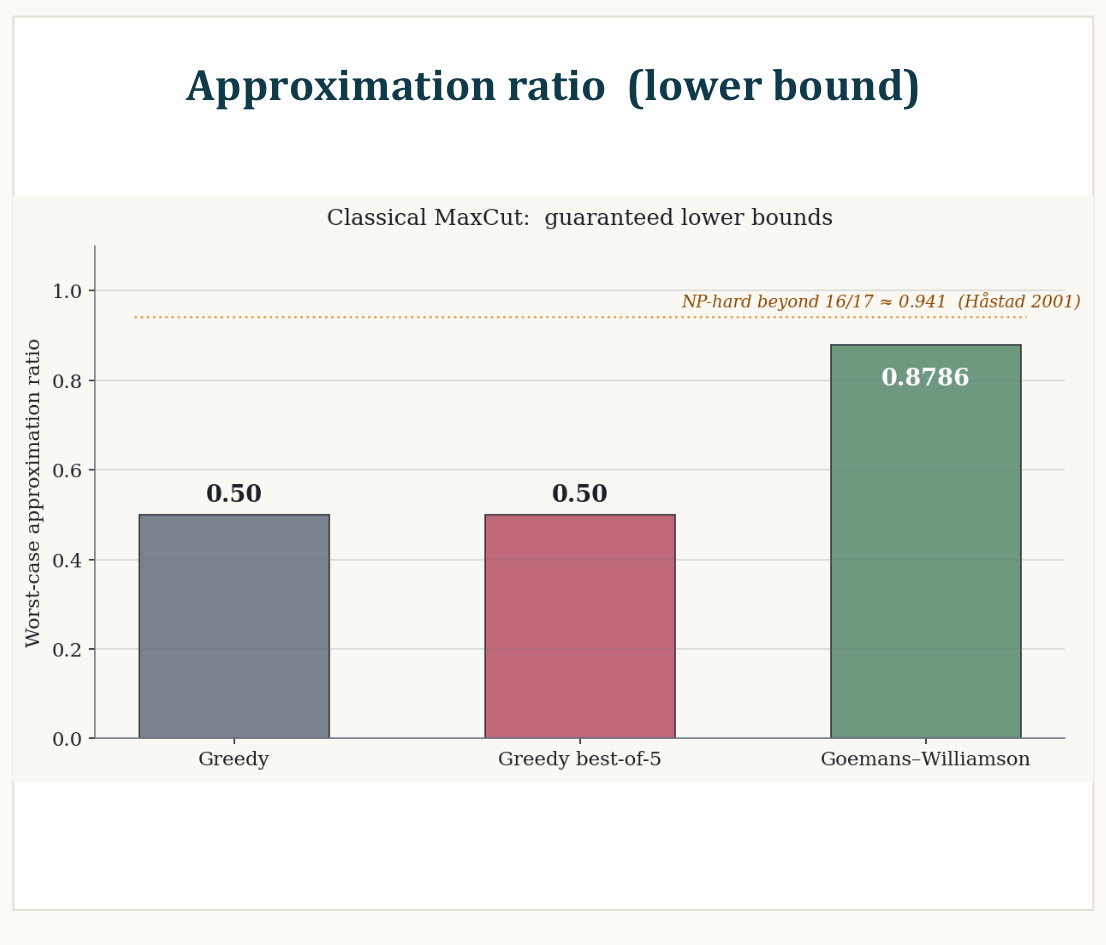
\includegraphics[width=\linewidth]{figs_from_pdf/gw_bars.png}
  \end{columns}
\end{frame}

% ============================================================
\section{Implementation}
% ============================================================

\begin{frame}{The hybrid loop}
  \framesubtitle{QAOA = quantum state preparation + classical optimiser}
  \begin{columns}[T,onlytextwidth]
    \column{0.55\textwidth}
      \textbf{Each iteration:}
      \begin{enumerate}
        \item Prepare $\ket{\psi_p(\bm\gamma,\bm\beta)}$ on the QPU.
        \item Measure $F_p = \langle\HC\rangle$ via repeated sampling.
        \item Send $F_p$ to a classical optimiser
              (COBYLA, L-BFGS-B, SPSA \ldots).
        \item Receive new $(\bm\gamma,\bm\beta)$, repeat until converged.
      \end{enumerate}

    \column{0.42\textwidth}
      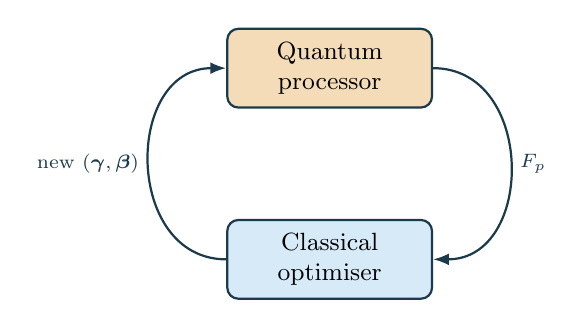
\begin{tikzpicture}[
          node distance=8mm and 6mm,
          box/.style={draw=NavyDeep,thick,rounded corners,
                      fill=NavyLite!30,minimum width=2.6cm,
                      minimum height=1.0cm,align=center,
                      font=\small},
          ar/.style={-{Latex[length=2mm]},thick,NavyDeep}]
        \node[box,fill=Mustard!30] (Q) {Quantum\\processor};
        \node[box,below=1.4cm of Q,fill=NavyLite!50] (C) {Classical\\optimiser};
        \draw[ar] (Q.east) .. controls +(1.3,0) and +(1.3,0)
            .. node[right,font=\scriptsize]{$F_p$} (C.east);
        \draw[ar] (C.west) .. controls +(-1.3,0) and +(-1.3,0)
            .. node[left,font=\scriptsize]{new $(\bm\gamma,\bm\beta)$} (Q.west);
      \end{tikzpicture}
  \end{columns}
\end{frame}

% --- C_4 explicit circuit -------------------------------------
\begin{frame}{Explicit circuit: $C_4$, depth $p=1$}
  \framesubtitle{The QAOA ansatz drawn out gate by gate}
  \begin{columns}[T,onlytextwidth]
    \column{0.22\textwidth}
      \centering
      \vspace{0.6em}
      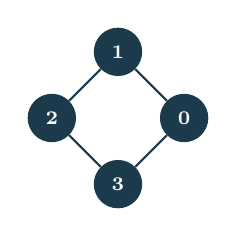
\begin{tikzpicture}[scale=0.7,
          v/.style={circle,draw=NavyDeep,fill=NavyDeep,
                    text=Cream,inner sep=1pt,minimum size=6mm,
                    font=\scriptsize\bfseries}]
        \node[v] (1) at ( 0, 1.2)  {1};
        \node[v] (2) at (-1.2, 0)  {2};
        \node[v] (0) at ( 1.2, 0)  {0};
        \node[v] (3) at ( 0,-1.2)  {3};
        \draw[NavyDeep,thick] (0)--(1)--(2)--(3)--(0);
      \end{tikzpicture}\\[2pt]
      {\footnotesize $C_4$ : 4 vertices,\\4 edges}\\[6pt]
      {\scriptsize $\gamma = 0.79,\ \beta = 0.39$}

    \column{0.76\textwidth}
      \centering
      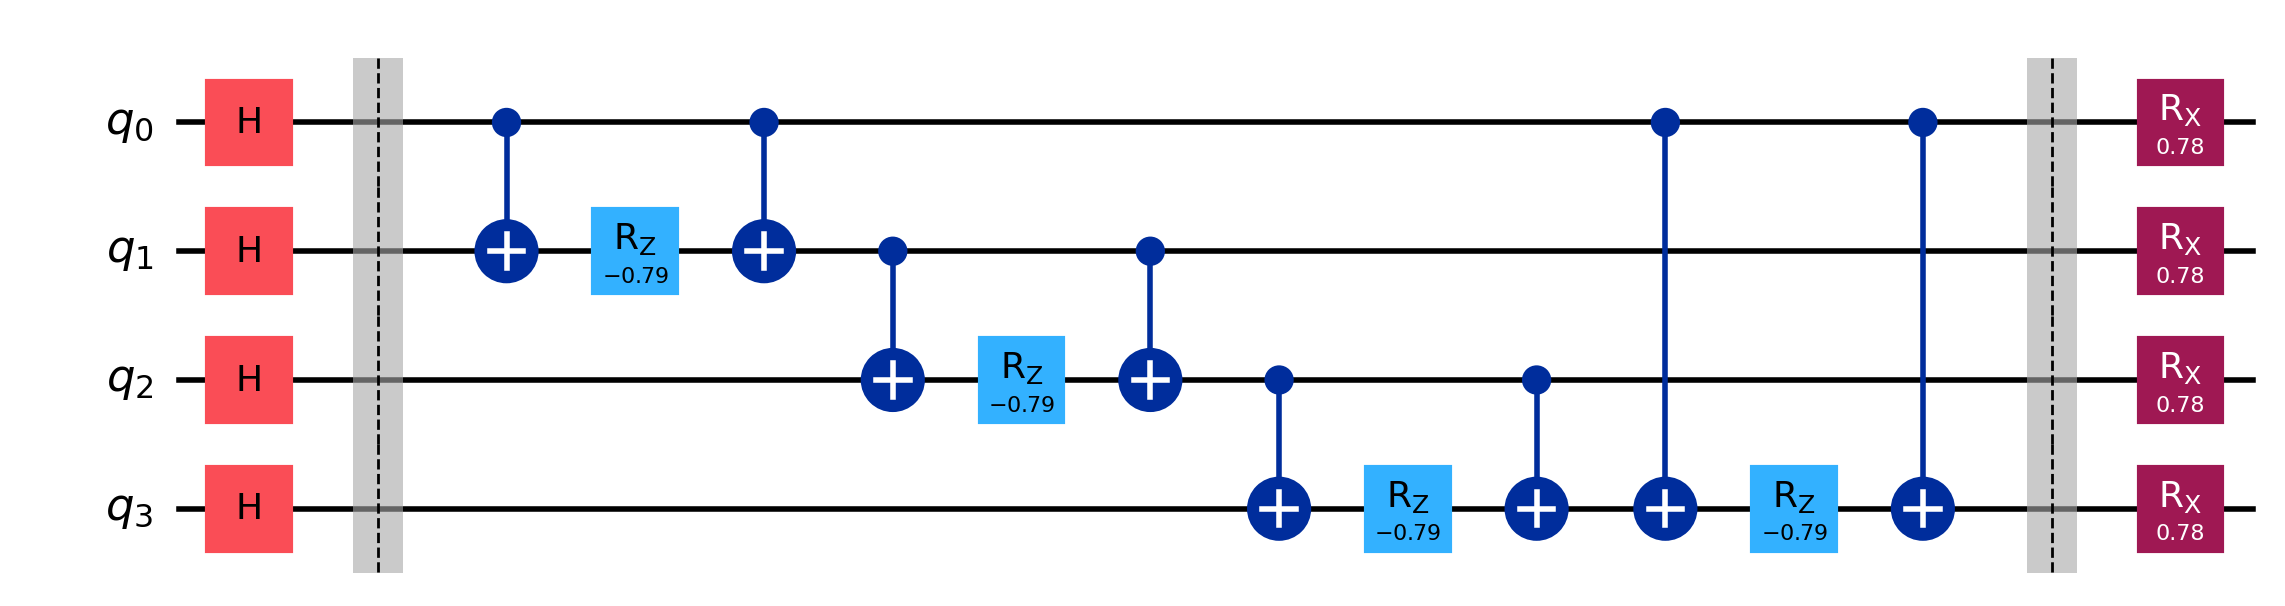
\includegraphics[width=\linewidth]{figs_from_pdf/c4_qaoa_circuit.png}
  \end{columns}

  \vspace{0.4em}
  \footnotesize
  Reading left $\rightarrow$ right: \textbf{(1)} $H^{\otimes 4}$ to
  prepare $\ket{+}^{\otimes 4}$,
  \;\textbf{(2)} four cost blocks $\UC(\gamma)$, one per edge,
  \;\textbf{(3)} four single-qubit $R_X(2\beta)$ gates as the mixer
  $\UB(\beta)$.
\end{frame}

% --- Why the circuit matches the ansatz -----------------------
\begin{frame}{How the circuit realises the ansatz}
  \framesubtitle{Per-edge $ZZ$ rotation and per-qubit $X$ rotation}
  \begin{columns}[T,onlytextwidth]
    \column{0.5\textwidth}
      \textbf{Cost unitary, edge by edge:}
      \[
        \UC(\gamma) = \!\!\prod_{(i,j)\in E}\!\! e^{-i\gamma(I-Z_iZ_j)/2}
      \]
      Drop the global phase $e^{-i\gamma/2}$ per term:
      \[
        e^{-i\gamma(I-Z_iZ_j)/2} \;\propto\; e^{+i\gamma\,Z_iZ_j/2}.
      \]
      Standard identity:
      \[
        e^{i\gamma Z_iZ_j/2}
        \;=\; \mathrm{CX}_{ij}\cdot R_Z(-\gamma)_j\cdot \mathrm{CX}_{ij}.
      \]
      One CX--$R_Z$--CX block per edge.

    \column{0.5\textwidth}
      \textbf{Mixer unitary, qubit by qubit:}
      \[
        \UB(\beta) \;=\; e^{-i\beta \sum_k X_k}
                   \;=\; \prod_{k} R_X(2\beta)_k.
      \]
      One $R_X(2\beta)$ per qubit --- no entangling gates.

      \vspace{0.8em}
      \textbf{Gate count for $C_4$, $p=1$:}
      \begin{itemize}\setlength{\itemsep}{1pt}
        \item $|E|=4$ edges $\Rightarrow$ 4 cost blocks
              (8 CX, 4 $R_Z$).
        \item $n=4$ qubits $\Rightarrow$ 4 $R_X$ + 4 $H$.
      \end{itemize}
  \end{columns}
\end{frame}

\begin{frame}{Choosing the classical optimiser}
  \framesubtitle{$C_{10}$ + 3 chords, $p=3$, statevector simulation}
  \centering
  \begin{tabular}{lllc}
    \toprule
    Optimiser    & Gradient            & Cost / step & Best for \\
    \midrule
    COBYLA       & none (trust-region) & $O(p)$      & shot-noise robust \\
    L-BFGS-B     & parameter-shift     & $2(|E|+n)p$ & exact gradient (sim) \\
    Nelder--Mead & none (simplex)      & $O(p)$      & fallback \\
    SPSA         & stochastic 2-eval   & $2$         & real hardware \\
    \bottomrule
  \end{tabular}

  \vspace{0.6em}
  \begin{block}{Our choice: L-BFGS-B (primary) + COBYLA (cross-check)}
    L-BFGS-B converges fastest on noiseless statevector via the exact
    per-edge parameter-shift gradient. Running COBYLA in parallel as a
    gradient-free baseline rules out optimiser-specific artefacts.
    SPSA would replace both on real hardware.
  \end{block}
\end{frame}

\begin{frame}{Optimiser comparison}
  \framesubtitle{Convergence behaviour on a representative instance}
  \vfill
  \makebox[\linewidth][c]{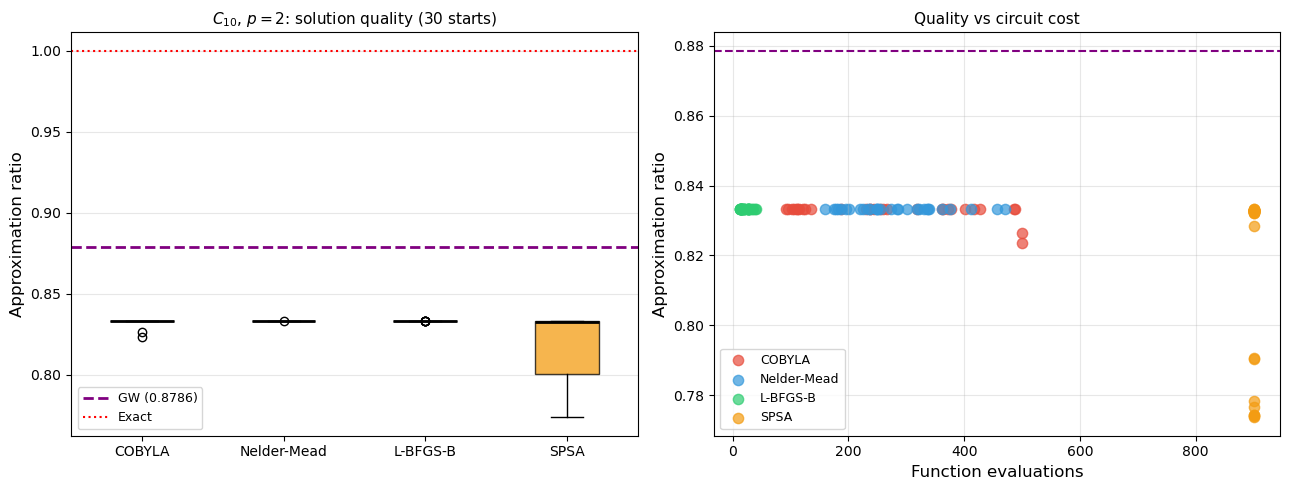
\includegraphics[width=1.15\linewidth]{../Implementation/figures/optimizer_comparison.png}}
  \vfill
\end{frame}

\begin{frame}{Warm start: initialise $p{+}1$ from the $p$-layer optimum}
  \framesubtitle{Random restarts at $p=3$ waste evaluations on distant local maxima}
  \begin{columns}[T,onlytextwidth]
    \column{0.45\textwidth}
      \textbf{Algorithm} (Zhou et al.\ 2020):
      \begin{enumerate}\small
        \item Optimise $p{=}1$ globally (random restarts).
        \item For $k = 2,\dots,p$:\\
              $\theta_0 \leftarrow (\bm\gamma^\star,\gamma^\star_{p-1})\,\Vert\,
                                  (\bm\beta^\star,\beta^\star_{p-1}) + \eta$\\
              Local optimise $F_k$ from $\theta_0$.
        \item Return final $(\bm\gamma^\star,\bm\beta^\star)$.
      \end{enumerate}

      \vspace{0.4em}
      \textbf{Intuition.} A $p$-layer optimum is already a good region
      of parameter space for $p{+}1$ layers — the extra layer with small
      $\gamma,\beta$ is nearly the identity.

    \column{0.55\textwidth}
      \centering
      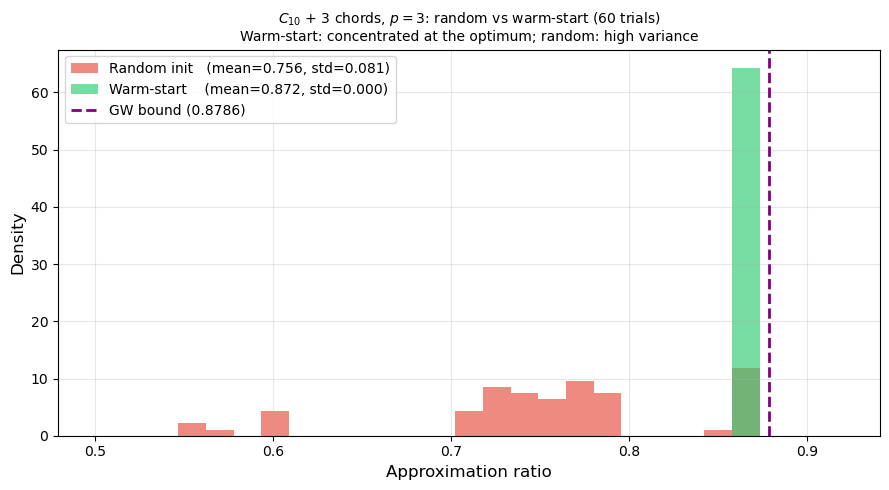
\includegraphics[width=\linewidth]{../Implementation/figures/warmstart_comparison.png}\\
      {\footnotesize\itshape Warm-start collapses the variance:
       std drops from 0.083/0.126 to 0.000.}
  \end{columns}
\end{frame}

% ============================================================
\section{Results}
% ============================================================

\begin{frame}{Problem instances}
  \framesubtitle{Three 10-vertex graphs --- $C_{10}$ has $\mathrm{MaxCut}=10$;\ \ $C_{10}$+3 chords and 3-regular both have $\mathrm{MaxCut}=13$}
  \vfill
  \makebox[\linewidth][c]{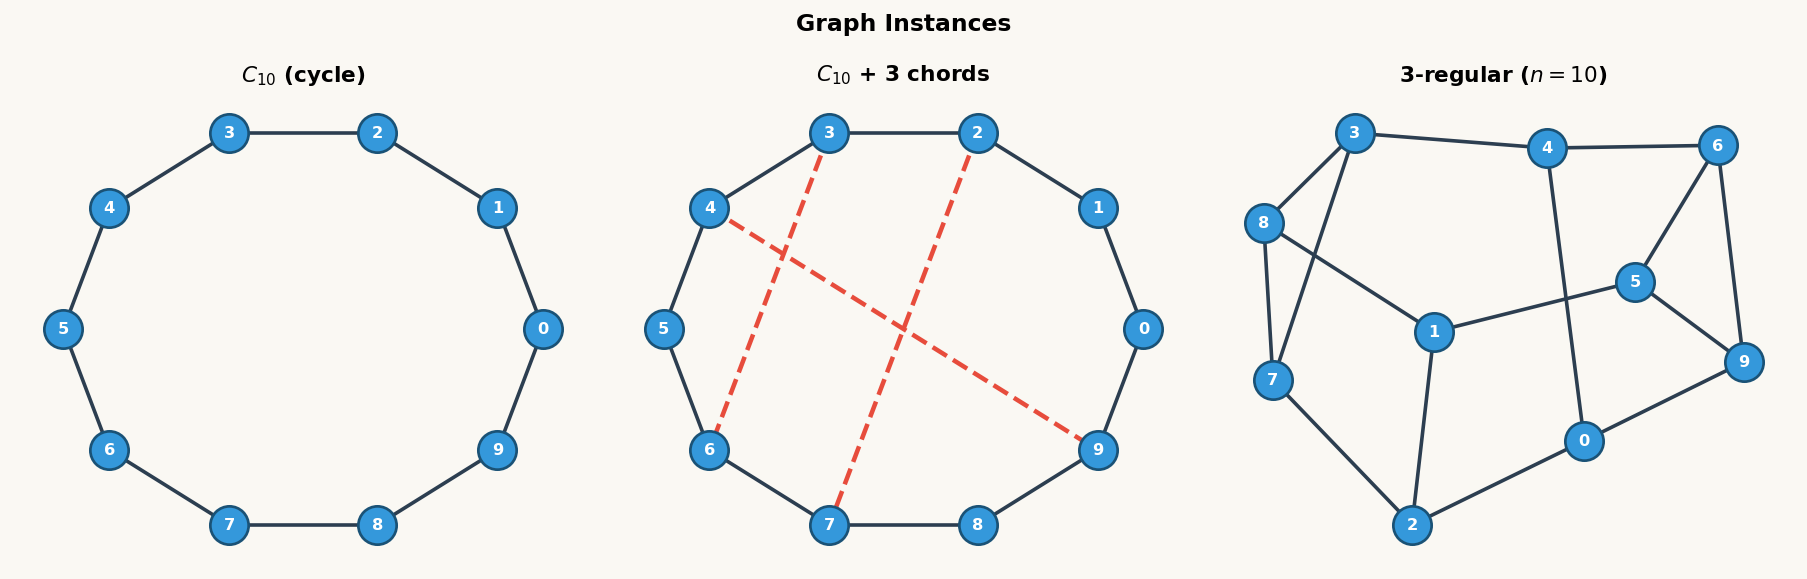
\includegraphics[width=1.15\linewidth]{../Implementation/exp_graphs.png}}
  \vfill
\end{frame}

\begin{frame}{Performance comparison}
  \framesubtitle{QAOA $p=3$ ties or surpasses Greedy best-of-5; GW remains the gold standard}
  \vfill
  \makebox[\linewidth][c]{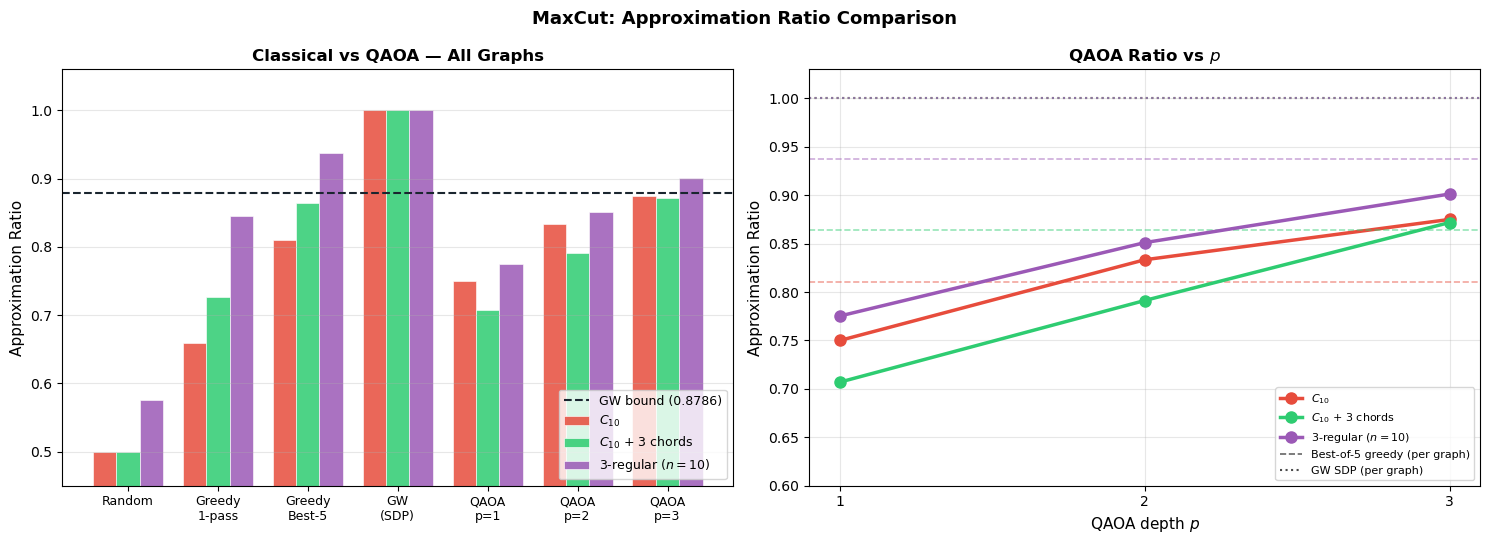
\includegraphics[width=1.15\linewidth]{../Results/figures/algorithm_comparison.png}}
  \vfill
\end{frame}

\begin{frame}{Approximation ratio versus depth}
  \framesubtitle{Monotone improvement, with diminishing returns past $p=3$. For all three graphs, $p=3$ approaches the GW bound (0.8786).}
  \vfill
  \makebox[\linewidth][c]{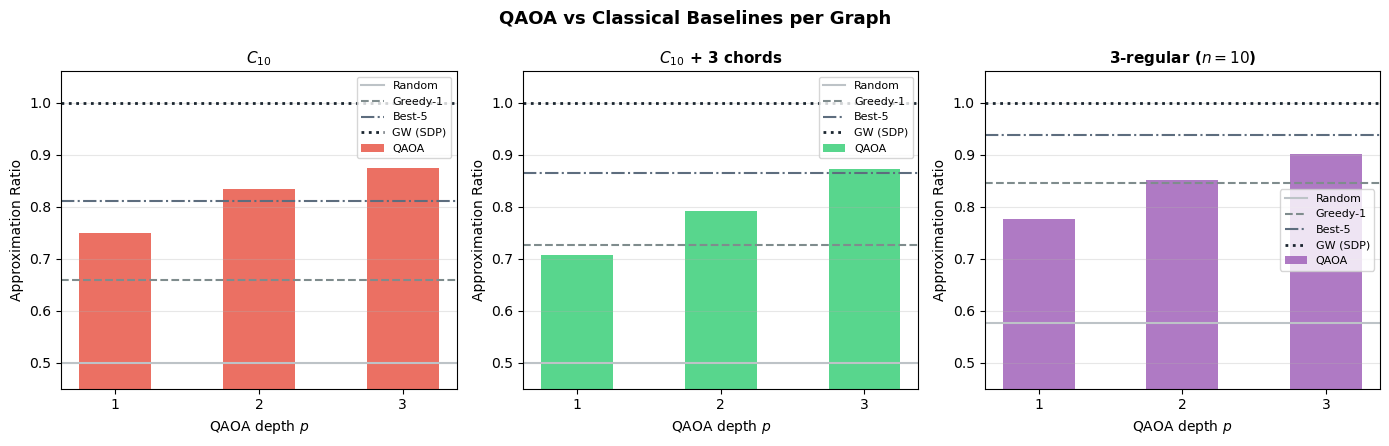
\includegraphics[width=1.15\linewidth]{../Results/figures/qaoa_depth_comparison.png}}
  \vfill
\end{frame}

\begin{frame}{Measurement distributions}
  \framesubtitle{The two MaxCut bitstrings dominate as $p$ grows}
  \begin{columns}[T,onlytextwidth]
    \column{0.7\textwidth}
      \centering
      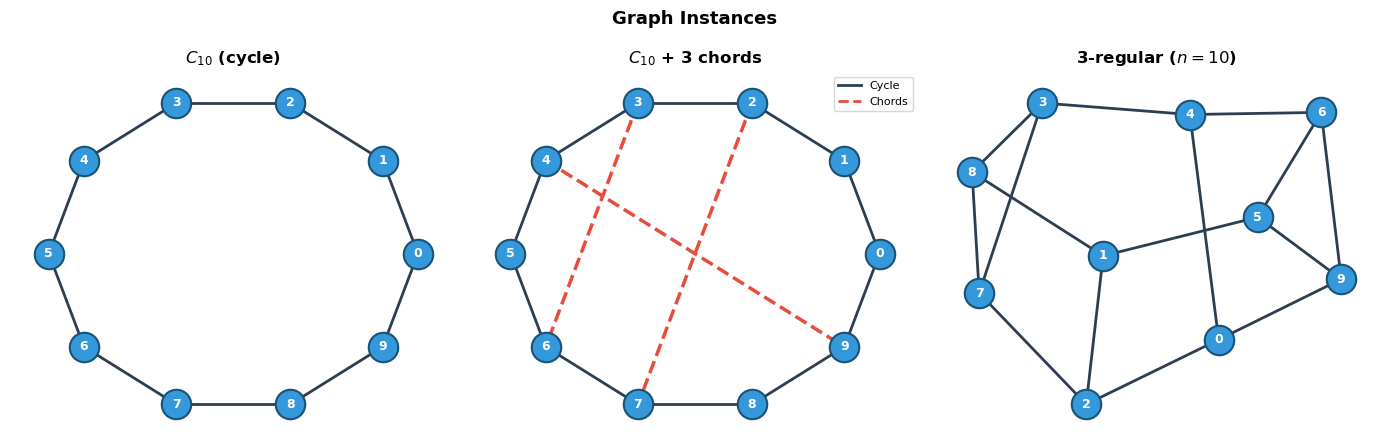
\includegraphics[width=\linewidth]{../Results/figures/graph_instances.png}
    \column{0.28\textwidth}
      \footnotesize
      \textbf{$C_{10}$:}\\
      $\ket{1010101010}$\\
      $\ket{0101010101}$\\[6pt]
      \textbf{$C_{10}$ + 3 chords:}\\
      same two states\\[6pt]
      \textbf{3-regular:}\\
      $\ket{1100110100}$\\
      $\ket{0011001011}$\\[6pt]
      Two solutions per graph because every cut has a $\mathbb{Z}_2$
      complement-symmetry $z \mapsto \bar z$.
  \end{columns}
\end{frame}

% --- 3-regular: best vs 2nd-best ------------------------------
\begin{frame}{3-regular: not just one peak}
  \framesubtitle{Sampled distribution shows the 2nd-best cut as the next-tallest peak}
  \begin{columns}[T,onlytextwidth]
    \column{0.62\textwidth}
      \centering
      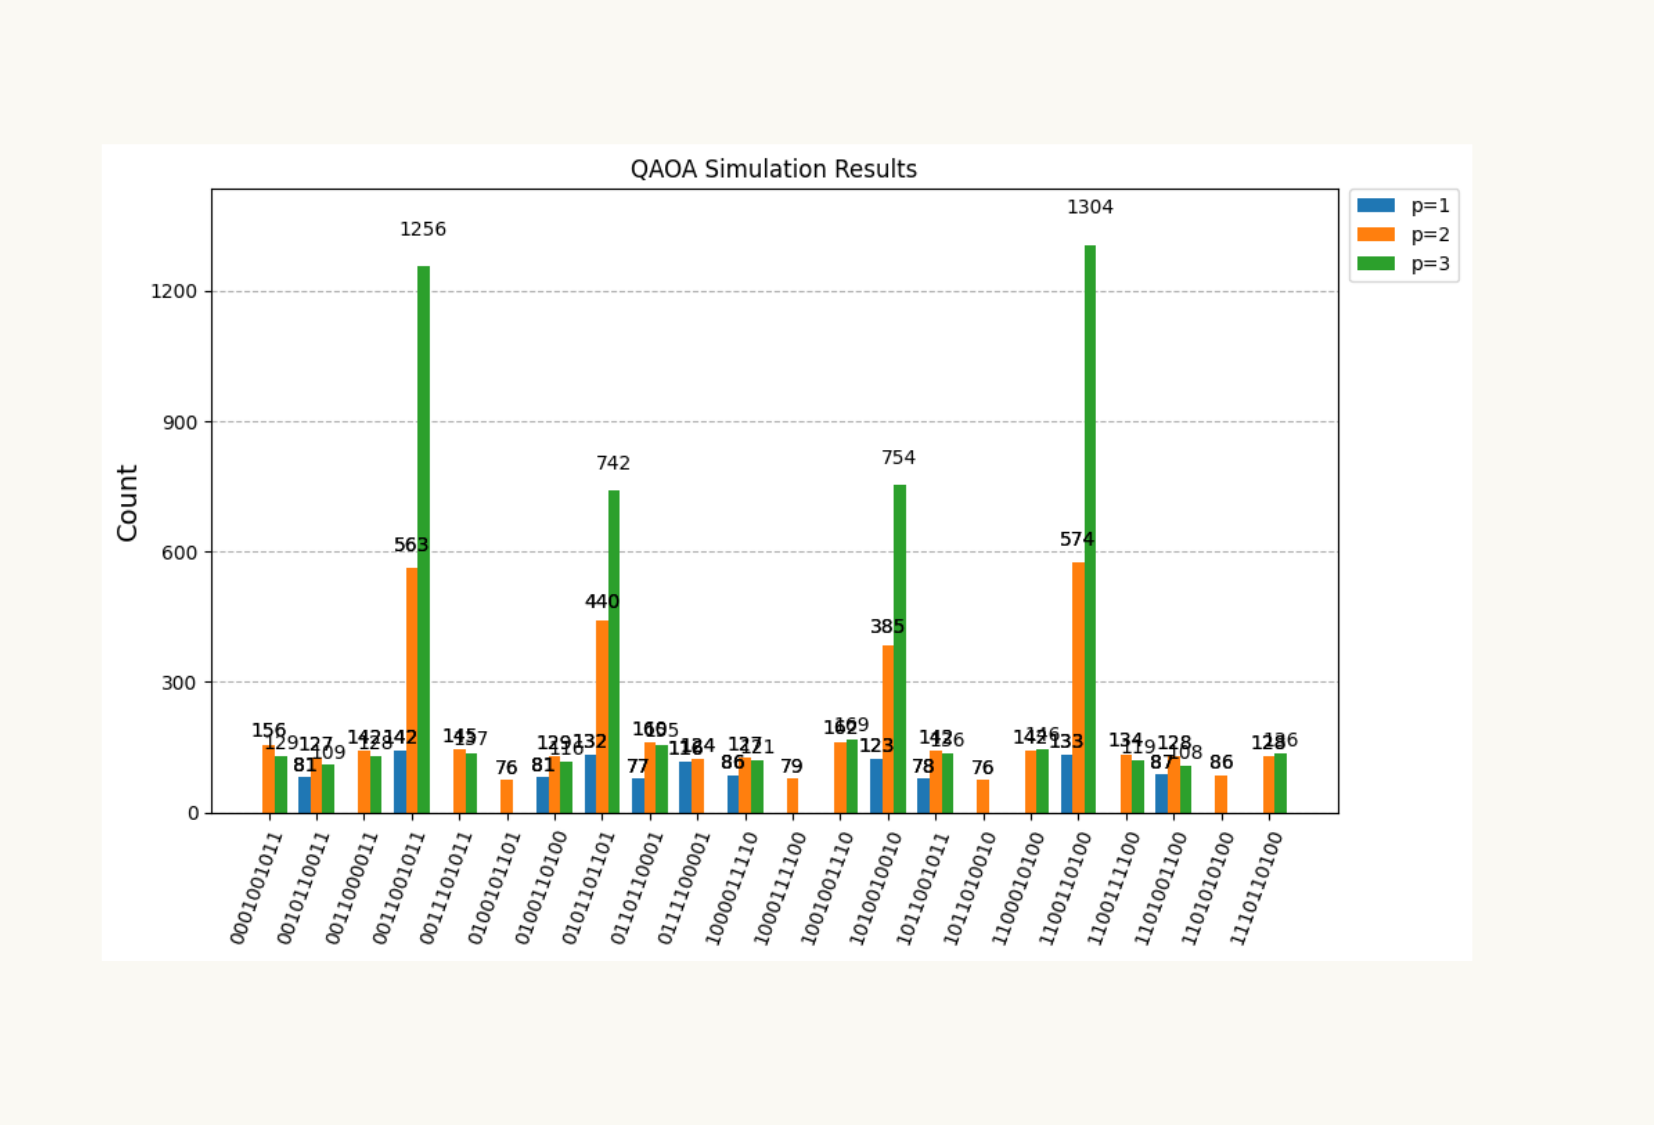
\includegraphics[width=\linewidth]{figs_from_pdf/3reg_hist.png}\\[2pt]
      {\footnotesize\itshape 4096 shots; $p=1$ blue, $p=2$ orange,
       $p=3$ green.}

    \column{0.36\textwidth}
      \centering
      \footnotesize\alert{cut $= 13$}\, (MaxCut)\\
      \scriptsize $\ket{1100110100},\,\ket{0011001011}$\\[1pt]
      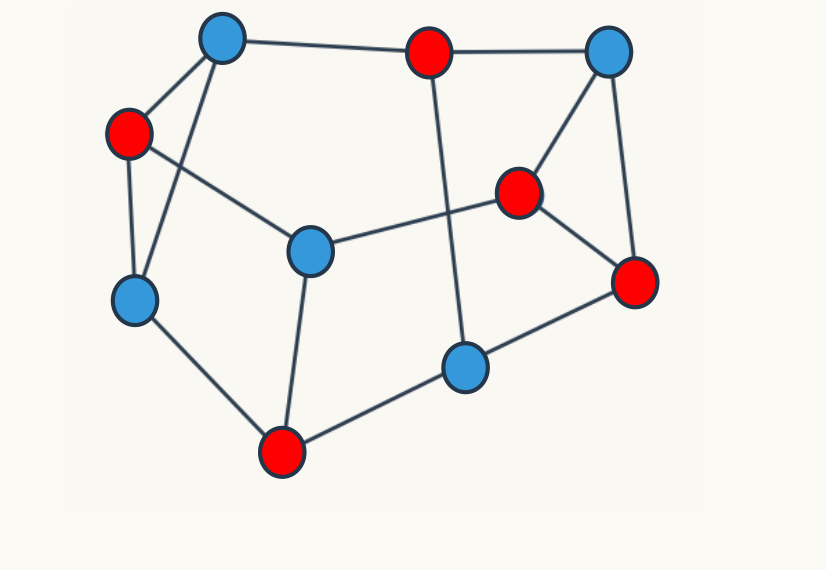
\includegraphics[height=3.0cm]{figs_from_pdf/3reg_best.png}\\[6pt]
      \footnotesize\alert{cut $= 12$}\, (2nd best)\\
      \scriptsize $\ket{0101101101},\,\ket{1010010010}$\\[1pt]
      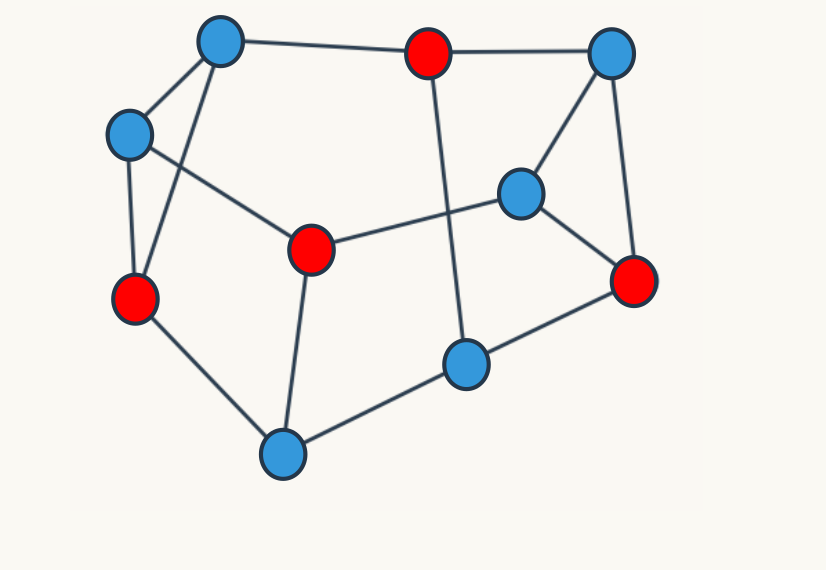
\includegraphics[height=3.0cm]{figs_from_pdf/3reg_second_best.png}
  \end{columns}
\end{frame}

% ----------------- NOISE -----------------------------------
\begin{frame}{Introducing noise}
  \framesubtitle{2-qubit depolarising channel with error probability $\pcx$}
  \begin{block}{After every CX gate}
    \[
      \mathcal{E}(\rho) \;=\; (1-\pcx)\,\rho
        \;+\; \frac{\pcx}{15}
              \!\!\sum_{P\in\{I,X,Y,Z\}^{\otimes 2}\setminus\{I^{\otimes 2}\}}\!\!
              P\rho P^{\dagger}
    \]
  \end{block}

  \begin{itemize}
    \item Single-qubit gates ($H$, $R_X$, $R_Z$) carry the same form
          with rate $\pcx/10$ (1Q fidelities are typically $10\times$
          better than 2Q).
    \item Total CX count $= 2p|E|$, so circuit fidelity decays as
          $(1-\pcx)^{2p|E|}$ --- noise grows with depth and graph size.
    \item We sweep $\pcx \in [0, 0.025]$.
  \end{itemize}
\end{frame}

\begin{frame}{Ratio degradation with CX error rate}
  \framesubtitle{Deeper circuits degrade faster --- they have $3\times$ more CX gates. Each curve uses the noiseless-optimal $(\bm\gamma,\bm\beta)$ from depth $p$.}
  \vfill
  \makebox[\linewidth][c]{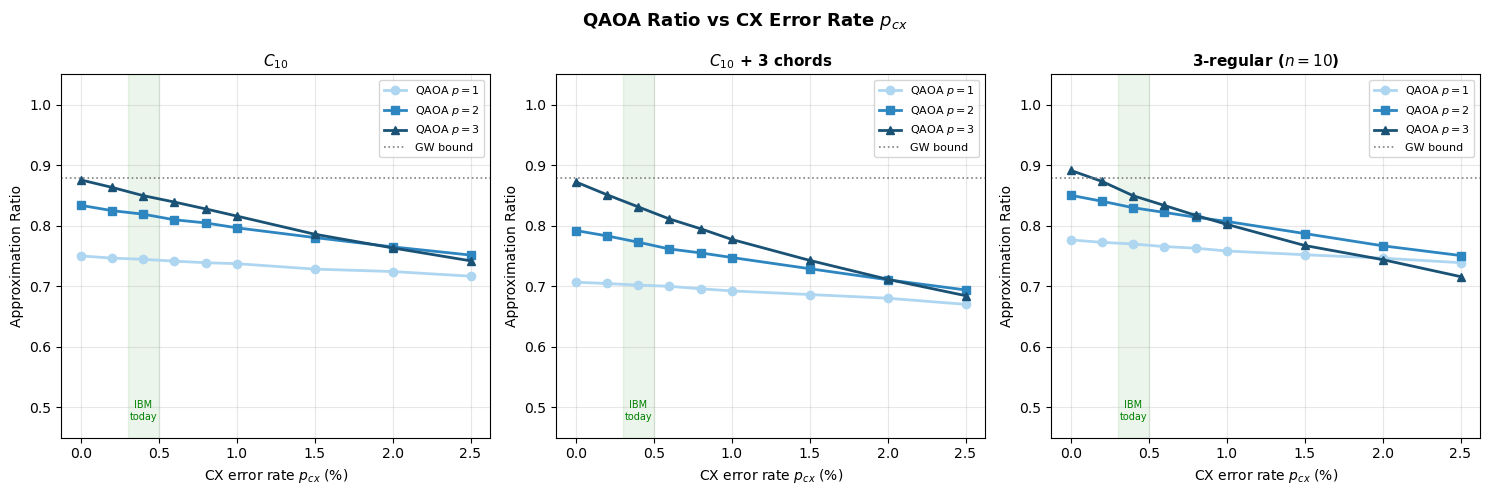
\includegraphics[width=1.15\linewidth]{../Results/figures/noise_degradation.png}}
  \vfill
\end{frame}

\begin{frame}{Crossover: when shallower beats deeper}
  \framesubtitle{Hardware noise dictates the optimal QAOA depth}
  \makebox[\linewidth][c]{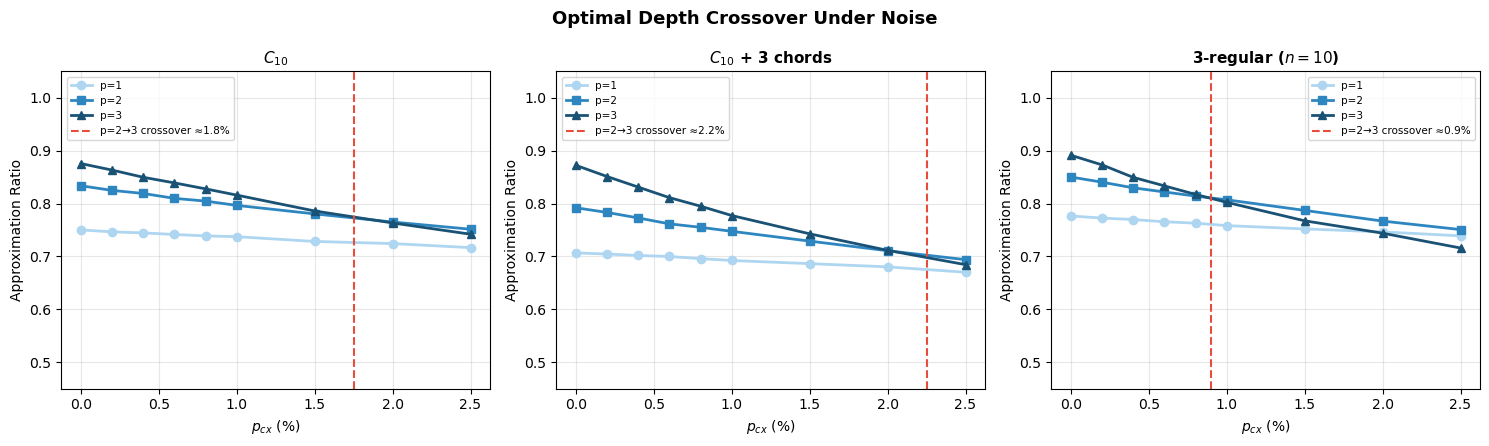
\includegraphics[width=1.12\linewidth]{../Results/figures/crossover_analysis.png}}\\[3pt]

  \begin{itemize}\small
    \item Total CX count $= 2p|E|$, so circuit fidelity decays as
          $(1-\pcx)^{2p|E|}$.
    \item Above $\pcx\!\approx\!1\%$, $p{=}1$ \textbf{outperforms} $p{=}3$
          on every graph tested.
    \item Reported median CX errors on superconducting hardware sit in
          the $0.5$--$1\%$ range — close to the crossover region.
  \end{itemize}
\end{frame}

% ============================================================
\begin{frame}[allowframebreaks]{References}
  \footnotesize
  \begin{itemize}
    \item Farhi, Goldstone, Gutmann.
          \emph{A Quantum Approximate Optimization Algorithm.}
          arXiv:1411.4028 (2014).
    \item Goemans, Williamson.
          \emph{Improved Approximation Algorithms for Maximum Cut and
          Satisfiability Problems Using Semidefinite Programming.}
          \mbox{JACM 42(6) (1995)}.
    \item Karp.
          \emph{Reducibility Among Combinatorial Problems.} (1972).
    \item H{\aa}stad.
          \emph{Some Optimal Inapproximability Results.}
          JACM 48(4) (2001).
    \item Khot, Kindler, Mossel, O'Donnell.
          \emph{Optimal Inapproximability Results for MAX-CUT and Other
          2-Variable CSPs.} JACM 54(3) (2007).
    \item McClean, Boixo, Smelyanskiy, Babbush, Neven.
          \emph{Barren Plateaus in Quantum Neural Network Training Landscapes.}
          Nature Commun. 9 (2018).
    \item Wang, Fontana, Cerezo, Sharma, Sone, Cincio, Coles.
          \emph{Noise-Induced Barren Plateaus in Variational Quantum Algorithms.}
          Nature Commun. 12 (2021).
    \item Cerezo, Sone, Volkoff, Cincio, Coles.
          \emph{Cost-Function-Dependent Barren Plateaus in Shallow
          Parametrized Quantum Circuits.}
          Nature Commun. 12 (2021).
    \item Bravyi, Kliesch, Koenig, Tang.
          \emph{Obstacles to Variational Quantum Optimization from
          Symmetry Protection.}
          arXiv:2110.14206 (2021).
    \item Zhou, Wang, Choi, Pichler, Lukin.
          \emph{Quantum Approximate Optimization Algorithm: Performance,
          Mechanism, and Implementation on Near-Term Devices.}
          Phys. Rev. X 10 (2020).
  \end{itemize}
\end{frame}

% ============================================================
\begin{frame}[plain]
  \centering
  \vfill
  {\Huge\bfseries\color{NavyDeep} Thanks for your attention!}\\[1em]
  {\color{Mustard}\rule{6em}{1.5pt}}\\[1em]
  {\large Sehong Park}\\[2pt]
  {\small Physics 565 / 656 \ \textperiodcentered\  Spring 2026}
  \vfill
\end{frame}

\end{document}
